\documentclass{article}
\usepackage{geometry,tikz}
\usetikzlibrary{shapes.geometric}
\geometry{paperheight=12cm,paperwidth=8cm,left=5pt,right=0pt,top=2pt,bottom=0pt}
\pagestyle{empty}
\begin{document}
\centering
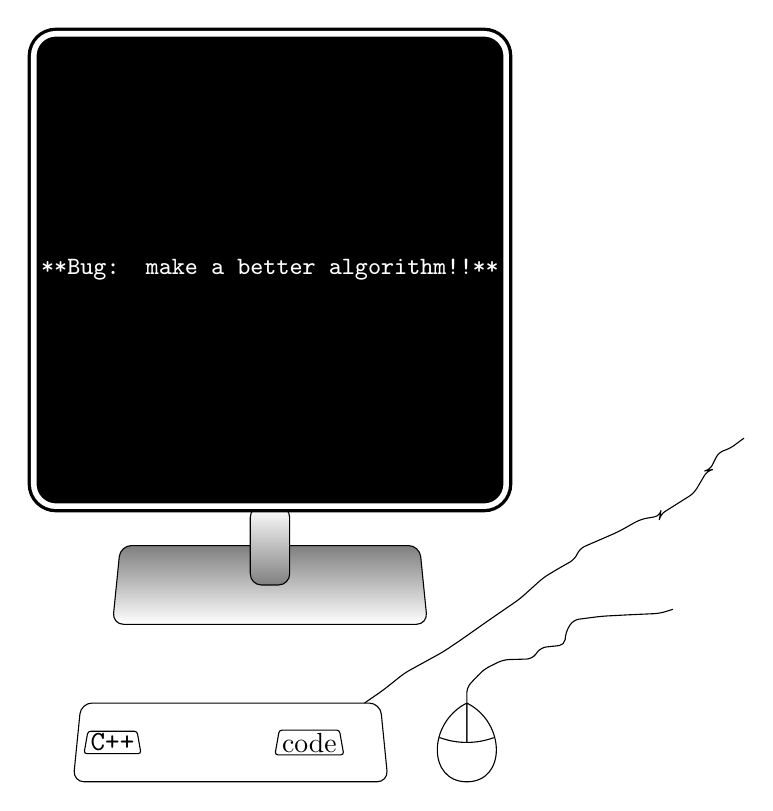
\begin{tikzpicture}
\shadedraw[rounded corners] (-2,-4.5) -- ++(4,0) -- ++(-0.1,1) -- ++(-3.8,0) -- cycle;
\shadedraw[rounded corners,bottom color=gray,top color=white] (-0.25,-3) rectangle ++(0.5,-1);
\draw[fill=black,double,double distance=2pt,very thick,rounded corners=8pt] (-3,-3) rectangle ++(6,6);
\node[white,font=\small\tt] at (0,0) {**Bug: make a better algorithm!!**};
%% keyboard
\draw[rounded corners] (-2.5,-6.5) -- ++(4,0) -- ++(-0.1,1) -- ++(-3.8,0) -- cycle;
\draw[rounded corners=2pt] (1.2,-5.5) \foreach \p in {1,...,20}{ -- ++(0.5*rnd,0.3*rnd)};
\foreach \touch/\coord in {{\texttt{C++}/{-2,-6}},{code/{0.5,-6}}}
        \node[shape=trapezium,trapezium left angle=80,trapezium right angle=80,
              inner sep=1pt,draw,rounded corners=1pt] at (\coord) {\touch};

%% mouse
  \draw (2.5,-6.5) .. controls ++(0.5,0) and ++(0.5,-0.25)  .. ++(0,1) 
        (2.5,-5.5) -- ++(0,-0.5) arc(-90:-70:1);
  \draw[xscale=-1] (-2.5,-6.5) .. controls ++(0.5,0) and ++(0.5,-0.25)  .. ++(0,1) 
                   (-2.5,-5.5) -- ++(0,-0.5) arc(-90:-70:1);
\draw[rounded corners=2pt] (2.5,-5.5) -- (2.5,-5.3) \foreach \p in {1,...,12}{ -- ++(0.4*rnd,0.2*rnd)};
\end{tikzpicture}
\end{document}
